\documentclass{article}
\usepackage{xeCJK}
\usepackage{amsmath}
\usepackage{amssymb}
\usepackage{mathrsfs}
\usepackage{bm}
\usepackage{graphicx}

\setlength{\parindent}{2em}
\usepackage{geometry}
\geometry{a4paper, left=2.54cm, right=2.54cm, top=3.18cm, bottom=3.18cm}

\begin{document}

\section{相位-取向关联的集群振子系统的动力学研究}

\textbf{$\Delta$ 聚焦点}
\begin{enumerate}
    \item 环态及其相变
    \item 环态的解域与相位同步的关系
    \item 数值结果的细致讨论, 分类
    \item 必要的理论分析与估计
\end{enumerate}

分析点
\subsection{单个粒子的运动问题(无相互作用)}

$$
\begin{cases}
	\begin{array}{c}
	\Delta x\left( t \right) =v\cos \theta \Delta t\\
	\Delta y\left( t \right) =v\sin \theta \Delta t\\
\end{array}\rightarrow \begin{array}{c}
	\dot{x}=v\cos \theta\\
	\dot{y}=v\sin \theta\\
\end{array}\\
	\dot{\theta}_i=\omega _i\rightarrow \theta _i\left( t \right) =\omega _it\\
	v=\sqrt{\dot{x}_{i}^{2}+\dot{y}_{i}^{2}}=v\left( constant \right)\\
\end{cases}
$$

运动半径 $=\ ?$

$$
\begin{cases}
	x_i\left( t \right) =x_i\left( 0 \right) -\frac{v}{\omega _i}\sin \omega _it\\
	y_i\left( t \right) =y_i\left( 0 \right) -\frac{v}{\omega _i}\cos \omega _it\\
\end{cases}
$$

$$
\Rightarrow \left( x_i-x_{i}^{0} \right) ^2+\left( y_i-y_{i}^{0} \right) ^2=\left( \frac{v}{\omega _i} \right) ^2
$$

每个粒子的运动轨迹是一个圆,圆心为 $\left( x_i^0,y_i^0 \right)$,半径为 $\frac{v}{\omega _i}$

\subsection{考虑相互作用$\lambda$,耦合距离$d_0$ ($\{A_ij\}$,注意是时变的)}

\begin{itemize}
    \item 看空间聚集过程
    \item 空间尺度也考虑进去
\end{itemize}

粒子数$N$,$L\times L\sim \sqrt{\frac{L\times L}{N}}\sim \frac{L}{\sqrt{N}}$

\begin{enumerate}
    \item 每个单粒子的运动空间尺度, $\cfrac{v}{\omega_i}$
    \item 耦合距离 $d_0$
    \item 粒子平均间距 $\cfrac{L}{\sqrt{N}}$
\end{enumerate}

$$
d_0\sim \frac{L}{\sqrt{N}}\rightarrow d_0\ll \frac{L}{\sqrt{N}}, d_0\gg \frac{L}{\sqrt{N}}
$$

低频粒子:$d_0\ll \frac{v}{\omega _i}$
高频粒子:$d_0\gg \frac{v}{\omega _i}$

在计算空间pattern同时,还要跟踪每个粒子的相速度$\dot{\theta}_i(t)$

\newpage

\section{局部耦合中跨边界坐标的调整}

\begin{figure}[htbp]
    \centering
    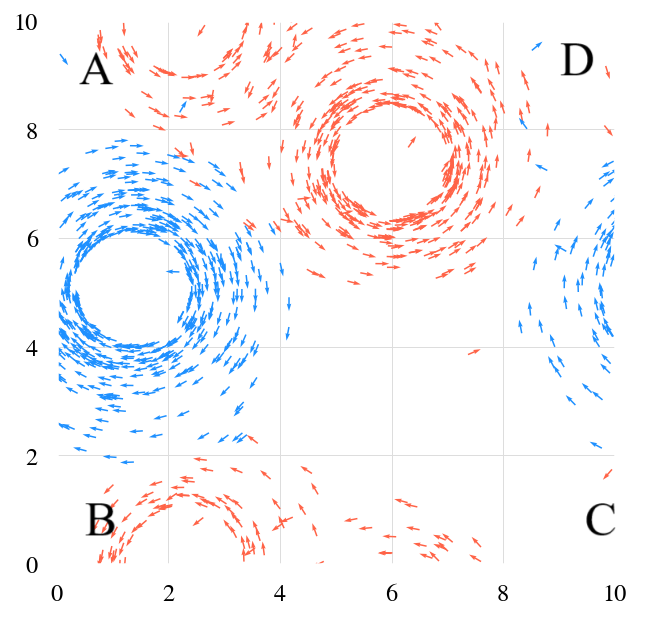
\includegraphics[width=0.4\textwidth]{./figs/fig1.jpg}
    \caption{跨边界坐标的调整}
    \label{fig:fig1}
\end{figure}

给定$(x_i, y_i)$, 对于任意的$(x_j, y_j)$, 做如下变换

$$
\bar{x}_j=\begin{cases}
	x_j,&		|x_i-x_j|\le L/2\\
	x_j+L,&		x_i-x_j>L/2\\
	x_j-L,&		x_j-x_i>L/2\\
\end{cases}
$$

$$
\bar{y}_j=\begin{cases}
    y_j,&		|y_i-y_j|\le L/2\\
    y_j+L,&		y_i-y_j>L/2\\
    y_j-L,&		y_j-y_i>L/2\\
\end{cases}
$$

其中,$L$为边界长度. 例如,对于\ref{fig:fig1}中的情况,以A为$(x_i, y_i)$时,B需调整纵坐标,D需调整横坐标,C需同时调整横纵坐标.

$\ $

原始距离为

$$
d_{ij}=\sqrt{(x_i-x_j)^2+(y_i-y_j)^2}
$$

变换后的距离为

$$
\bar{d}_{ij}=\sqrt{(x_i-\bar{x}_j)^2+(y_i-\bar{y}_j)^2}
$$

下证$\bar{d} \le d_{ij}$:

$ $

对于$(x_i-x_j)^2, (x_i-\bar{x}_j)^2$, 若$x_i\ne \bar{x}_j$,有

$$
\begin{array}{l}
	(x_i-\bar{x}_j)^2-(x_i-x_j)^2\\
	=\left( x_j\pm L-x_i \right) ^2-(x_i-x_j)^2\\
	=L^2\pm 2L\left( x_j-x_i \right)\\
	=\left\{ \begin{matrix}
	L^2+2L\left( x_j-x_i \right) ,&		x_i-x_j>5\\
	L^2-2L\left( x_j-x_i \right) ,&		x_j-x_i>5\\
\end{matrix} \right.\\
	<L^2-10L\\
	=0, \left( L=10 \right)\\
\end{array}
$$

即

$$
(x_i-\bar{x}_j)^2<(x_i-x_j)^2, \left( L=10, x_i\ne \bar{x}_j \right)
$$

同理可证

$$
(y_i-\bar{y}_j)^2<(y_i-y_j)^2, \left( L=10, x_i\ne \bar{x}_j \right)
$$

综上有

$$
\bar{d}_{ij}=\sqrt{(x_i-\bar{x}_j)^2+(y_i-\bar{y}_j)^2}\le \sqrt{(x_i-x_j)^2+(y_i-y_j)^2}=d_{ij}
$$

当且仅当$x_i=\bar{x}_j$且$y_i=\bar{y}_j$时,取等号.

因此

$$
\begin{aligned}
	D_{ij}&=\min \left\{ \sqrt{(x_i-\bar{x}_j)^2+(y_i-\bar{y}_j)^2},\sqrt{(x_i-x_j)^2+(y_i-y_j)^2} \right\}\\
	&=\sqrt{(x_i-\bar{x}_j)^2+(y_i-\bar{y}_j)^2}\\
\end{aligned}
$$


\end{document}